\chapter{Implementation of Privacy Protection Measures}
\section{Privacy Policy}

In complience legal requirements of the Data Protection Directive (cf. Section \ref{EUDIR}) we include the following
Privacy Policy on our Mobile Application and Website.

\begin{quote}
\tt \small
\textbf{Privacy Policy}\\
==============

\textbf{What Personal Information do we Collect?}\\
The Live+Gov Service Center stores the following personal information:\\
- Name\\
- Email Address\\

The Mobile Sensor Collection Application collects the following data from your mobile phone:\\
- Sensor Data from Accelerometer (50Hz)\\
- Sensor Data from GPS sensors (~every 30 sec)\\
- Daily Human Activities (walking, standing, sitting, etc.) (every 30sec)\\
- Used Service Lines (bus, train, tram) (every 2 minutes)\\

All collected data is transferred to our data center.

\textbf{Which processing is applied to the data?}\\
We process Accelerometer samples on the Mobile device in order to extract human activities.
We process GPS coordinates on the Live+Gov server to extract the currently used service lines.

The stored information is used to produce aggregate reports.
These reports are based on anonymized data that do not allow the reconstruction of the routes of individual persons at a given point in time.

\textbf{When is the data deleted?}\\
The full data-set will be stored until January 2015.

Afterwards we will delete Names and Email addresses and anonymize
the sensor data and processing results.  The anonymized data will
be used by the the Consortium Partners for research purposes.

\textbf{For which purposes is the data collected?}\\
The collected data will be used for personalization of user experience of the mobile application.
Moreover, we will analyize travel patterns in the Helsinki Urban region for general research and for improvement and optimization of the
infrastructure provided by HSL.

\textbf{Identity of Data Controller}\\
The data is controlled by Heinrich Hartmann <hartmann@uni-koblenz.de>

The following organizations have access to the collected data:
\begin{enumerate}
\item University of Koblenz-Landau
\url{http://www.uni-koblenz-landau.de/}\\
Universitätsstraße 1\\
56070 Koblenz

\item Mattersoft
\url{http://www.mattersoft.fi/}
Hämeenkatu 13, 33100 Tampere, Finland\\
+358 10 3225000

\item Centre for Research and Technology Hellas (CERTH)
\url{http://mklab.iti.gr/contact}\\
6th km Charilaou-Thermi Road\\
P.O. Box 60361,\\
57001 Thermi-Thessaloniki, Greece
\end{enumerate}

\textbf{Access to Stored Data}\\
All personal data can be accessed at our Privacy Dashboard at
\url{http://liveandgov.uni-koblenz.de/trial/dashboard}

There you have the possibility to:\\
- View all recordings made\\
- View the raw data collected for each recording\\
- Download the data for each recording\\
- Delete records

\textbf{Collaboration with Third Parties}\\
The raw data is not shared with any parties external to the Live+Gov Consortium.

Aggregated report based on anonymized data are disclosed to officials at HSL \url{http://www.hsl.fi/} and might be made
public in the form of a blog post or research article.  These aggregated reports show distributions of all routes that
have been collected in the system and do not allow to infere the location of a single user at a given point in time.

\textbf{Consent}\\
I have read and understood the above privacy policy and agree that my data is collected and processed accordingly.
\end{quote}

\section{Processing Journal}
* name of the controller
* purpose of processing
* description of the data categories
* recipients of the data if disclosed
* transfer to third countries
* description of security of processing

The journal is available for anybody to access via Email.

Reporting to Data Protection Authority (Bundesamt für Datenschutz)?

\section{Privacy Dashboard}
TODO: Add description of dashboard. With relation to 7C's of Privacy.

\begin{figure}
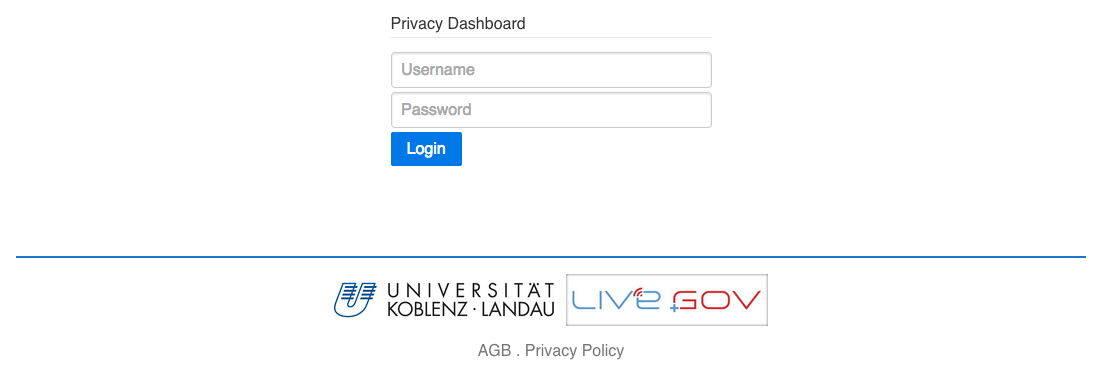
\includegraphics[width=\textwidth]{screenshots/login.png}
\caption{Live+Gov Privacy Dashboard Login}
\end{figure}

\begin{figure}
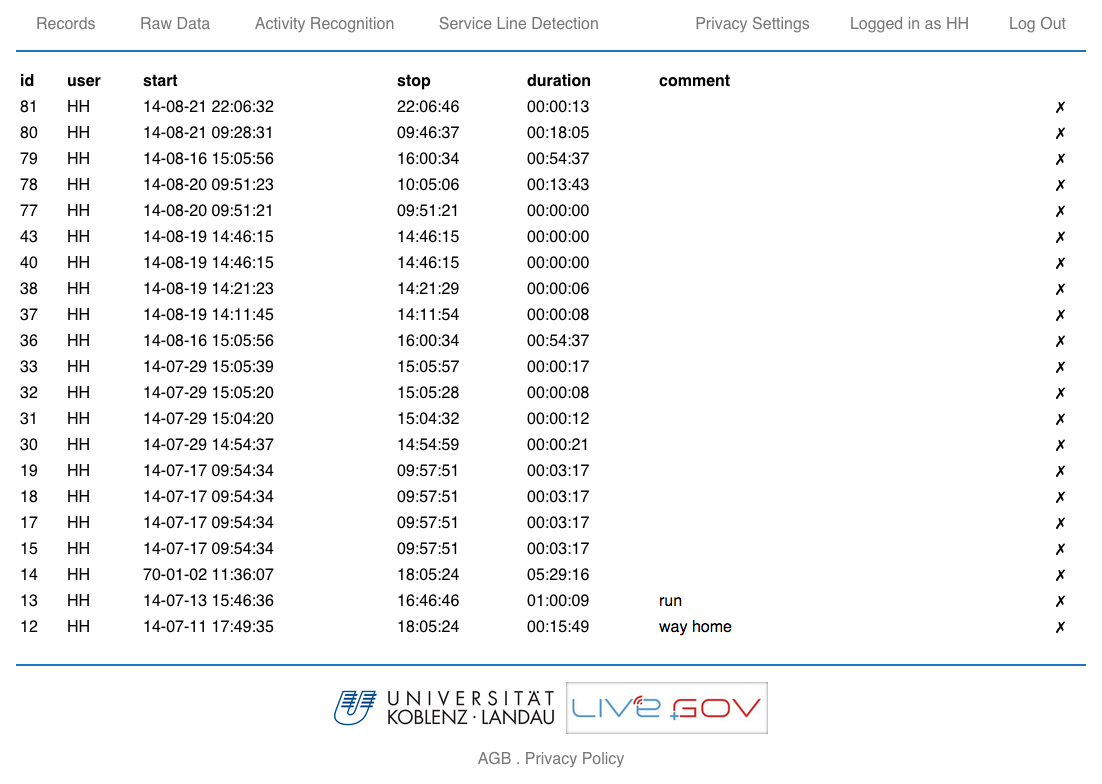
\includegraphics[width=\textwidth]{screenshots/recordings.png}
\caption{Live+Gov Privacy Dashboard Recording Overview}
\end{figure}

\begin{figure}
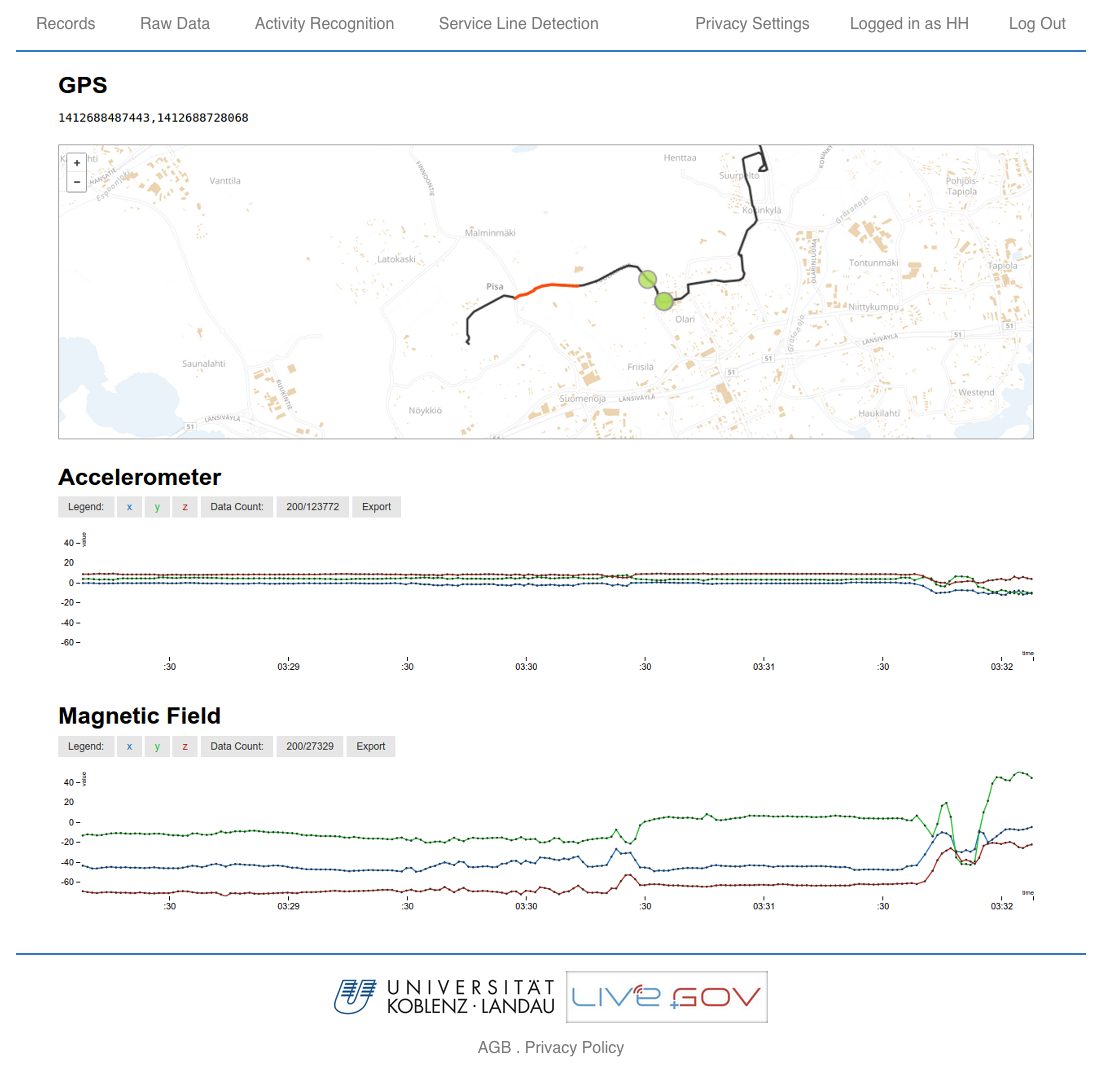
\includegraphics[width=\textwidth]{screenshots/raw.png}
\caption{Live+Gov Privacy Dashboard Raw Data View}
\end{figure}

\begin{figure}
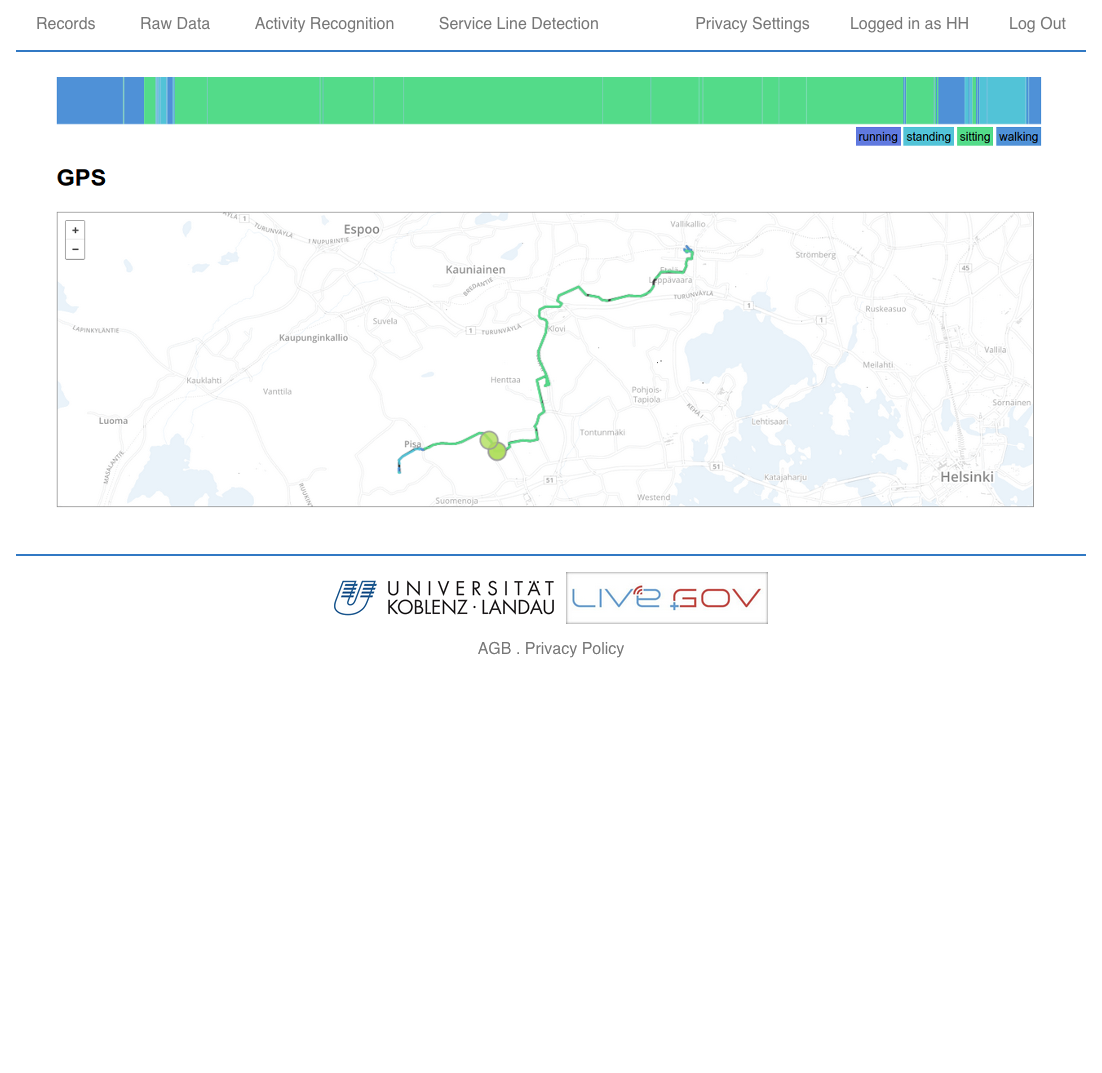
\includegraphics[width=\textwidth]{screenshots/processed.png}
\caption{Live+Gov Privacy Dashboard Processed Data View}
\end{figure}

\section{Transfer Encryption (HTTPS/SSL)}
\begin{figure}
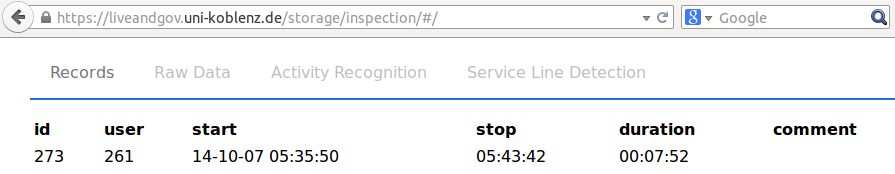
\includegraphics[width=\textwidth]{screenshots/HTTPS.png}
\caption{HTTPS connection to Privacy Dashboard}
\end{figure}

\section{Database Access Policies}
Access rules for data controller and processor.
Data Processing Journal.
Python script for deletion of data when it is older than a given date.

\section{Anonymization of trips}
Privacy by Design: We do never collect name and email address in our DB.
Python script that deletes user information from trip.
% Python script that reomves precise date information, only day of week.

\section{K-Anonymity of GPS routes}
Python script that deletes all parts of journeys that have are not near to at least k other journeys.

TODO: Insert Literature Reference.
TODO: Add screenshots.

\section{Randomization of GPS data}
Python Script that adds random noise to GPS data.
